\documentclass[11pt,a4paper]{article}
\usepackage[T1]{fontenc}
\usepackage[margin=2.3cm]{geometry}
\usepackage{amsmath,amssymb}
\usepackage{graphicx}
\usepackage[dvipsnames]{xcolor}
\usepackage{enumitem}
\usepackage[colorlinks=true,linkcolor=blue,urlcolor=blue]{hyperref}
\setlength{\parskip}{0.6em}
\setlength{\parindent}{0pt}
\begin{document}

\begin{center}{\LARGE\bfseries opentrafficsignal}\\[0.4em]{\large Time a traffic-signal junction to cut waiting and queues, in three sessions.}\\[0.2em]\small PAN IIT OSS explainer \textbullet{} middle school to higher secondary (levels 2-4)\end{center}

\section*{Why this exists}
A traffic signal does not move cars; it decides who waits. This explainer shows how that decision creates queues and delay, using a few cars per second, a saturation flow and a green time, so you can reason about it and test it yourself.

\section*{The end goal}
Time a traffic-signal junction to cut waiting and queues. The end goal is timing a signalised junction to cut waiting and queues, as traffic engineers do: choose a cycle, share the green, and decide when a signal should react to the traffic. The models here are simplified and educational, not a design tool.

\section*{How the three sessions build up}
\begin{enumerate}[nosep]
\item \textbf{Session 1: Two phases, one queue} (Level 1, conceptual interactive model, 60 min).
\item \textbf{Session 2: Delay from cycle time, green split and flow} (Level 2, mathematical engineering model, 75 min).
\item \textbf{Session 3: A junction simulator, checked against the formula} (Level 3, simulation and validation, 90 min).
\end{enumerate}

\section{Session 1: Two phases, one queue}

\subsection*{A. Real-world problem}
At a four-way junction two roads cross, and only one may drive at a time. The signal alternates: green for road A while road B waits at red, then amber, then the other way round. Cars keep arriving on the waiting road, so a queue builds; when the light turns green the queue drains. Drivers feel this as waiting; a city feels it as queues that block the previous junction. How long does the queue get, and how long does it take to disappear? This is a simplified educational model, not a traffic engineering tool.

\subsection*{B. Concept and theory}
Each road gets a green time g, then an amber time a (3 s here; cars do not leave on amber, so it is lost time), then waits while the other road goes. For two equal phases the cycle time is C = 2 (g + a). Cars arrive at a steady rate q cars per second. On green they leave at the saturation flow s, the most cars per second that can leave a queue; about 0.5 cars per second per lane is a typical textbook value (about 1800 cars per hour), and real values vary with the road. A road is not green for r = C - g seconds. In that time q r cars arrive and none leave, so the queue peaks at q r. On green the queue shrinks at the speed s - q, so it needs q r / (s - q) seconds to vanish. If it does not vanish before the green ends, the leftover grows every cycle. The largest steady arrival rate a road can serve is its capacity s g / C.

\begin{itemize}[nosep]
\item g: green time of one road (s)
\item a: amber time (3 s here) (s)
\item C: cycle time, 2 (g + a) (s)
\item r: time a road is not green, C - g (s)
\item q: arrival rate (cars per second)
\item s: saturation flow (typical value 0.5 per lane) (cars per second)
\item capacity: largest steady arrival rate, s g / C (cars per second)
\end{itemize}

\begin{equation*}
C = 2\,(g + a),\qquad r = C - g
\end{equation*}

\begin{equation*}
Q_{\max} = q\,r\quad\text{(cars waiting at the end of red)}
\end{equation*}

\begin{equation*}
t_{\text{clear}} = \frac{q\,r}{s - q}\quad\text{(seconds of green needed to empty the queue)}
\end{equation*}

\begin{equation*}
\text{capacity} = \frac{s\,g}{C},\qquad \text{the queue clears every cycle only if } q < \text{capacity}
\end{equation*}

\begin{center}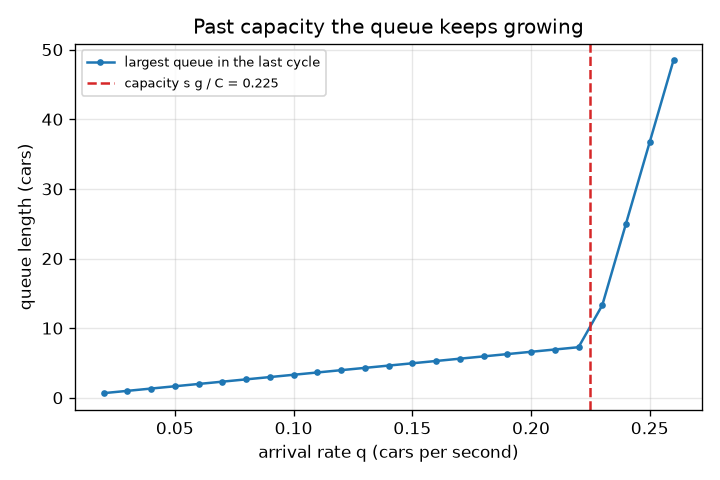
\includegraphics[width=0.85\linewidth]{figures/s01_queue_vs_rate.png}\\\small Largest queue against arrival rate: it takes off at the capacity 0.225 cars per second.\end{center}

\subsection*{E. Worked example}
A road has green g = 27 s, amber 3 s and cars arrive at q = 0.15 cars per second (s = 0.5). Find the cycle time, the red time, the peak queue, the time to clear it and the capacity. Does the queue clear every cycle?
\begin{enumerate}[nosep]
\item C = 2 (27 + 3) = 60 s and r = C - g = 60 - 27 = 33 s.
\item Peak queue = q r = 0.15 x 33 = 4.95 cars.
\item Cars leave at 0.5 and arrive at 0.15, so the queue shrinks at 0.35 cars per second: t\_clear = 4.95 / 0.35 = 14.14 s.
\item 14.14 s is less than the 27 s of green, so the queue clears with 12.9 s to spare.
\item Capacity = s g / C = 0.5 x 27 / 60 = 0.225 cars per second, above 0.15, which agrees.
\end{enumerate}
\textbf{Answer.} C = 60 s, r = 33 s, peak queue 4.95 cars, cleared after 14.14 s of green; capacity 0.225 cars per second, so the queue clears every cycle. The simulation in lesson.py gives a peak of 4.93 cars.

\subsection*{F. Questions}
\begin{enumerate}[nosep]
\item \textbf{Conceptual.} On green, cars leave at 0.5 cars per second, yet the queue shrinks more slowly than that. Why? What happens to the shrinking speed as the arrival rate gets closer to 0.5?
\item \textbf{Numerical.} Road A has green 20 s, amber 3 s and q = 0.10 cars per second (s = 0.5). Find C, r, the peak queue, the time to clear it and the capacity. Sanity check: is the answer in the right units?
\item \textbf{Graph and simulation interpretation.} In the second figure (largest queue against arrival rate for g = 27 s), the points rise in a straight line and then take off. At what arrival rate does it happen, and what is happening to the queue after that?
\item \textbf{Design and optimisation challenge.} Design: two equal roads each receive q = 0.18 cars per second. Choose the green time g (a whole number of seconds, amber 3 s) so that the queue clears every cycle and the peak queue is at most 6 cars. Which g would you pick and why?
\end{enumerate}

\section{Session 2: Delay from cycle time, green split and flow}

\subsection*{A. Real-world problem}
A main road carries 0.20 cars per second and a side road 0.10. The cycle is 60 seconds. If both roads get the same green, the main road is nearly full while the side road is half empty. How many seconds of green should each get, and how long will drivers wait on average? Too little for the busy road and its queue never ends; too little for the quiet road and a few drivers wait a very long time. We turn the queue of Session 1 into a formula for the average delay per car. This is a simplified educational model; real junction timing follows national guidance and measured data.

\subsection*{B. Concept and theory}
Use effective green g (the time cars really leave) and effective red r = C - g. The flow ratio is y = q / s, the green ratio is lam = g / C, the capacity is s lam and the degree of saturation is x = q / (s lam). Plot cumulative arrivals (a straight line of slope q) and cumulative departures (flat on red, slope s while a queue exists on green). The vertical gap is the queue; the horizontal gap is a car's wait; the area between the curves is the total waiting time per cycle. It is a triangle with height q r (the peak queue) and base r s / (s - q) (the time until the queue is gone), so its area is q r\textasciicircum{}2 s / (2 (s - q)). Dividing by the q C cars that pass in one cycle gives Webster's uniform delay d = C (1 - lam)\textasciicircum{}2 / (2 (1 - q/s)) seconds per car. It assumes even arrivals and x \textless{}= 1; random surges add a further term in practice. For two roads sharing a cycle, the effective greens add up to C - L, where L is the lost time per cycle (6 s here, from two 3 s ambers). The quantity to minimise is the total delay rate q1 d1 + q2 d2 (car-seconds of waiting per second), or the average delay (q1 d1 + q2 d2) / (q1 + q2). Webster's rule of thumb for the cycle is C = (1.5 L + 5) / (1 - Y), where Y is the sum of the critical flow ratios of the phases, and the green is shared in proportion to the flow ratios.

\begin{itemize}[nosep]
\item C: cycle time (s)
\item g: effective green of one approach (s)
\item q: arrival rate (cars per second)
\item s: saturation flow (typical value 0.5 per lane) (cars per second)
\item y: flow ratio q / s (no unit)
\item lam: green ratio g / C (no unit)
\item x: degree of saturation q C / (g s) (no unit)
\item d: uniform delay per car (s)
\item L: lost time per cycle (6 s) (s)
\item Y: sum of critical flow ratios (no unit)
\end{itemize}

\begin{equation*}
y=\frac{q}{s},\qquad \lambda=\frac{g}{C},\qquad x=\frac{q}{s\lambda}=\frac{qC}{sg}
\end{equation*}

\begin{equation*}
\text{area per cycle}=\frac12\,(q r)\left(\frac{r s}{s-q}\right),\qquad d=\frac{\text{area}}{qC}
\end{equation*}

\begin{equation*}
d=\frac{C\,(1-g/C)^2}{2\,(1-q/s)}\quad(x\le 1)
\end{equation*}

\begin{equation*}
\min_{g_1}\ \frac{q_1 d_1(g_1)+q_2 d_2(C-L-g_1)}{q_1+q_2}\quad\text{subject to } x_1\le x_{\max},\ x_2\le x_{\max}
\end{equation*}

\begin{equation*}
C_{\text{Webster}}=\frac{1.5L+5}{1-Y},\qquad g_i=(C-L)\,\frac{y_i}{Y}
\end{equation*}

\begin{center}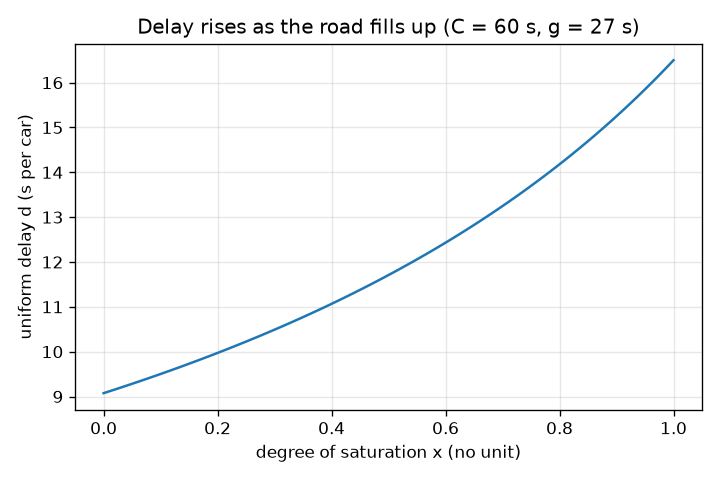
\includegraphics[width=0.85\linewidth]{figures/s02_delay_vs_saturation.png}\\\small Uniform delay against degree of saturation for C = 60 s, g = 27 s: slow rise, then steep.\end{center}

\subsection*{E. Worked example}
With C = 60 s, effective green 27 s for each road (54 s in total, L = 6 s), s = 0.5 cars per second, find x and d for the main road (q = 0.20) and the side road (q = 0.10), and the average delay per car of the junction.
\begin{enumerate}[nosep]
\item Green ratio lam = 27 / 60 = 0.45 for both roads, so (1 - lam)\textasciicircum{}2 = 0.55\textasciicircum{}2 = 0.3025.
\item Main road: x = 0.20 x 60 / (27 x 0.5) = 12 / 13.5 = 0.889 (below 1, the queue clears).
\item Main road delay: d = 60 x 0.3025 / (2 (1 - 0.20/0.5)) = 18.15 / (2 x 0.6) = 15.125 s.
\item Side road: x = 0.10 x 60 / 13.5 = 0.444 and d = 18.15 / (2 (1 - 0.2)) = 18.15 / 1.6 = 11.344 s.
\item Average delay per car = (0.20 x 15.125 + 0.10 x 11.344) / 0.30 = (3.025 + 1.134) / 0.30 = 13.86 s.
\end{enumerate}
\textbf{Answer.} Main road x = 0.889, d = 15.125 s; side road x = 0.444, d = 11.344 s; average delay 13.86 s per car. Giving the main road 40.7 s and the side road 13.3 s lowers it to 11.02 s with both x at most 0.9.

\subsection*{F. Questions}
\begin{enumerate}[nosep]
\item \textbf{Conceptual.} Why does the uniform delay contain the square of the red fraction, (1 - g/C)\textasciicircum{}2, and not just the red fraction? What does a longer red do to the queue and to each car's wait?
\item \textbf{Numerical.} A road has C = 90 s, effective green 40 s and q = 0.15 cars per second (s = 0.5). Find the degree of saturation and the uniform delay. Check the units and decide whether the formula applies.
\item \textbf{Graph and simulation interpretation.} In the delay-against-split graph (C = 60 s, q1 = 0.20, q2 = 0.10), the curve is not defined for splits below about 44 percent or above about 78 percent. Why, and where is the minimum?
\item \textbf{Design and optimisation challenge.} Design: with C = 60 s, q1 = 0.20 and q2 = 0.10 cars per second, choose the effective greens (total 54 s) that minimise the average delay with both degrees of saturation at most 0.9. Compare with the equal split and the proportional split. What would you check before using it?
\end{enumerate}

\section{Session 3: A junction simulator, checked against the formula}

\subsection*{A. Real-world problem}
Real cars do not arrive at neat intervals; they come in random bunches. Does the tidy formula of Session 2 still describe them? Does a signal that reacts to the queues beat a fixed timetable? And what happens when more cars arrive than the junction can ever serve? We answer with a simulator whose every car has an arrival time and a leaving time, so we can count the waiting exactly. This is a simplified educational model, not a traffic engineering tool; real signal timing needs measured data, safety checks and professional review.

\subsection*{B. Concept and theory}
Arrivals are a Poisson process with average rate q: the gaps between cars are exponentially distributed, and a seeded random generator makes every run repeatable. For validation we also use perfectly even arrivals, which match the assumptions of the formula. Time advances in steps of 0.5 s. In each step new cars join their queue, the controller says which phase is green or amber, and cars of a green approach leave at the saturation flow s (a credit grows by s dt per step and a car leaves each time it reaches 1; the first car of a green leaves at once). Delay of a car = time it crosses the stop line minus its arrival time; cars still waiting at the end count their delay so far. The fixed controller follows a timetable. The actuated controller keeps green while the phase still has a queue (up to a maximum of 45 s) and hands over when that queue is empty and the other phase waits, but not before a minimum of 8 s. Checks: (1) conservation, arrived = departed + still waiting; (2) with even arrivals the simulated delay should be close to the uniform delay; (3) the sum of all car delays equals the area under the queue curve (Little's law). Webster's cycle C = (1.5 L + 5) / (1 - Y) is a classic rule of thumb for the cycle that minimises delay including random effects; the delay is nearly flat around it.

\begin{itemize}[nosep]
\item q: arrival rate (cars per second)
\item s: saturation flow (typical value 0.5 per lane) (cars per second)
\item dt: time step (s)
\item C, g: cycle time and green time (s)
\item d: average delay per car (s)
\item Q\_max: largest queue on any approach (cars)
\item Y: sum of the critical flow ratios of the two phases (no unit)
\item L: lost time per cycle (6 s) (s)
\end{itemize}

\begin{equation*}
P(\text{gap} > t)=e^{-q t}\quad\text{(Poisson arrivals: exponential gaps)}
\end{equation*}

\begin{equation*}
N_{\text{arrived}}=N_{\text{departed}}+N_{\text{waiting}}\quad\text{(conservation of cars)}
\end{equation*}

\begin{equation*}
\sum_i d_i \;\approx\; \int Q(t)\,dt\quad\text{(total delay = area under the queue curve)}
\end{equation*}

\begin{equation*}
d_{\text{uniform}}=\frac{C(1-g/C)^2}{2(1-q/s)},\qquad C_{\text{Webster}}=\frac{1.5L+5}{1-Y}
\end{equation*}

\begin{equation*}
\text{queue growth rate}\approx q-\frac{s\,g}{C}\quad(q>\text{capacity})
\end{equation*}

\begin{center}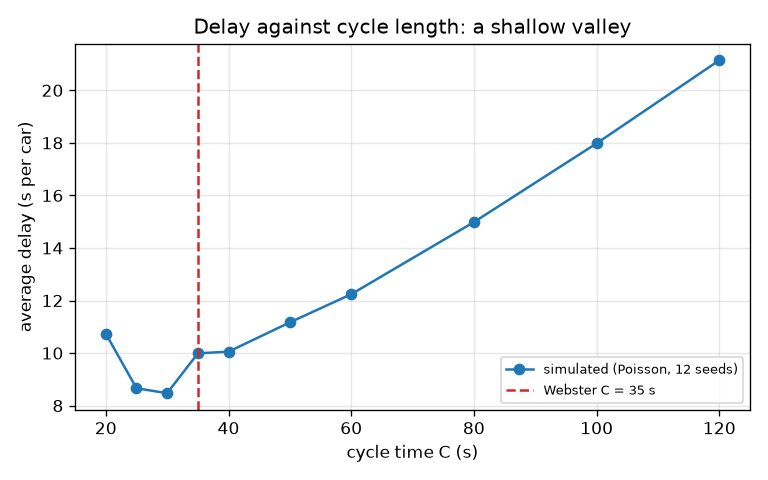
\includegraphics[width=0.85\linewidth]{figures/s03_delay_vs_cycle.png}\\\small Average delay against cycle length: a shallow valley with its minimum near 30 s; Webster says 35 s.\end{center}

\subsection*{E. Worked example}
Two roads with q = (0.20, 0.10) cars per second, s = 0.5, a fixed plan of 27 s + 27 s of green (C = 60 s). Validate the simulator: (1) even arrivals against the formula of Session 2, (2) conservation, (3) Little's law. Then show how random arrivals change the answer.
\begin{enumerate}[nosep]
\item Formula from Session 2: 13.86 s average delay per car (15.125 s for the main road, 11.344 s for the side road).
\item Simulation with even arrivals over 2 hours: 13.44 s, 3.1 percent below the formula (the car-by-car departures differ slightly from a smooth fluid). The largest queue is 7 cars, in line with q r = 0.2 x 33 = 6.6.
\item Conservation: 1440 + 720 cars arrived, 1433 + 720 departed and 7 + 0 are still waiting, so the gap arrived - departed - waiting is 0 for both roads.
\item Little's law: the car delays add up to 29033 car-seconds and the area under the queue curve is 28495, 1.9 percent apart (the queue is sampled once per step).
\item Poisson arrivals, 12 seeds: 19.50 s average delay and 18.5 cars largest queue, against 13.44 s and 7 cars for even arrivals: the random bunches add about 6 s per car.
\end{enumerate}
\textbf{Answer.} The simulator reproduces the formula within 3.1 percent for even arrivals, conserves cars exactly and obeys Little's law within 2 percent. With random arrivals the same plan gives 19.5 s instead of 13.4 s: the formula is the delay of a perfectly regular road and is a lower bound for a random one.

\subsection*{F. Questions}
\begin{enumerate}[nosep]
\item \textbf{Conceptual.} Even and Poisson arrivals have the same average flow, yet Poisson arrivals give more delay and longer queues. Why? Could random arrivals ever give less delay than even ones on average?
\item \textbf{Numerical.} A two-phase junction has q = (0.25, 0.15) cars per second, s = 0.5 and L = 6 s. Find Y, Webster's cycle and the two greens. One simulation run reports 720 cars arrived on road 2 and 719 departed. How many are still waiting?
\item \textbf{Graph and simulation interpretation.} In the delay-against-cycle graph (q = 0.20 and 0.10, Webster C = 35 s), describe the curve on the left and on the right of its minimum and say what the simulation finds as the best cycle.
\item \textbf{Design and optimisation challenge.} Design: the junction of the worked example (q = 0.20 and 0.10) was timed with Webster's cycle for its own demand (C = 35 s). In the evening the demand rises to 1.4 times (q = 0.28 and 0.14). The simulation gives 68.5 s average delay with the old plan. Re-time it with Webster's formula, give the new cycle and greens, and say when you would prefer an actuated rule.
\end{enumerate}

\section{Real-world mini-project}
\textbf{Time a junction from its traffic counts.} The city gives you 15-minute counts for a four-way junction, every approach with two lanes (saturation flow 1.0 car per second per approach, typical value) and 3 seconds of amber: north 360 cars, east 270, south 315, west 225. North and south share phase 0, east and west share phase 1. Turn the counts into flows, find the critical flow ratio of each phase, time the junction with \texttt{webster\_plan}, and compare it with a fixed plan of 27 s and 27 s of green and with the actuated rule over 12 seeds.

\section{The path ahead}
\begin{enumerate}[nosep]
\item \textbf{Session 4: The random delay term.} A formula for the total average delay that combines the uniform term and a random term, validated against the simulator.
\item \textbf{Session 5: Adaptive timing for a swinging rush hour.} A simulator with demand that changes every few minutes and a smarter adaptive rule (for example one that compares queue pressure of both phases).
\item \textbf{Session 6: Three phases: a protected turn.} A controller and simulator with three phases (the shipped one supports two).
\item \textbf{Session 7: A green wave between two junctions.} Two signals 400 m apart, cars travelling at 10 m/s, linked by an offset.
\item \textbf{Session 8: Fit the model to real counts.} A script that reads counts per minute from a CSV, estimates q and s and reports predicted delay and queue.
\end{enumerate}

\section{Answers and hints}

\subsection*{Session 1}
\begin{enumerate}[nosep]
\item \textbf{Conceptual.} Hint: Cars keep arriving while the queue is draining. Solution: New cars join the back of the queue while old ones leave the front, so the queue shrinks at the difference s - q, not at s. As q approaches s the shrinking speed approaches zero and the clearing time q r / (s - q) grows without limit: a road that is almost always demanding the full saturation flow can never get rid of its queue.
\item \textbf{Numerical.} Hint: C = 2 (g + a); peak = q r; clear time = peak / (s - q); capacity = s g / C. Solution: C = 2 (20 + 3) = 46 s and r = 46 - 20 = 26 s. Peak queue = 0.10 x 26 = 2.6 cars. Clear time = 2.6 / (0.5 - 0.1) = 6.5 s. Capacity = 0.5 x 20 / 46 = 0.217 cars per second. Units: cars per second times seconds gives cars; cars divided by cars per second gives seconds. 6.5 s is less than the 20 s green and 0.10 is below 0.217, so the queue clears every cycle.
\item \textbf{Graph and simulation interpretation.} Hint: Compare with the red dashed line, s g / C. Solution: The take-off is at the capacity s g / C = 0.225 cars per second. Below it the largest queue is q r = 33 q, a straight line through the origin with slope 33 s. Above it the arrivals per cycle exceed what one green can serve, so some cars are left over every cycle and the queue grows from one cycle to the next without limit.
\item \textbf{Design and optimisation challenge.} Hint: Two conditions: capacity s g / C above 0.18, and q r at most 6 where r = g + 6. Solution: Capacity condition: 0.5 g / (2 g + 6) \textgreater{} 0.18 gives g \textgreater{} 7.7, so g \textgreater{}= 8 (but g = 8 leaves almost no spare: capacity 0.182). Peak condition: 0.18 (g + 6) \textless{}= 6 gives g \textless{}= 27.3, so g \textless{}= 27. Any g from 8 to 27 meets both; a sensible choice is 15 to 20 s: g = 15 gives peak 3.8 cars and capacity 0.208 (a 16 percent margin), g = 20 gives peak 4.7 cars and capacity 0.217. Trade-off: shorter greens mean shorter queues but waste more of the cycle in amber; longer greens raise capacity but make the waiting road wait longer.
\end{enumerate}

\subsection*{Session 2}
\begin{enumerate}[nosep]
\item \textbf{Conceptual.} Hint: Think of the triangle: both its height and its base depend on r. Solution: The peak queue is q r (the height of the triangle) and the time it takes to clear is proportional to r as well (the base). The total waiting time is the area, which is proportional to r times r. Per car, the delay therefore grows with r squared divided by the cycle length. Doubling the red roughly quadruples the delay per car.
\item \textbf{Numerical.} Hint: x = q C / (g s); d = C (1 - g/C)\textasciicircum{}2 / (2 (1 - q/s)). Solution: x = 0.15 x 90 / (40 x 0.5) = 13.5 / 20 = 0.675 (no unit), below 1, so the formula applies. d = 90 x (1 - 40/90)\textasciicircum{}2 / (2 (1 - 0.15/0.5)) = 90 x 0.3086 / 1.4 = 19.84 s per car. Units: seconds x (no unit) / (no unit) = seconds. Sanity check: the red lasts 50 s, a car arriving at a random moment of the red waits 25 s on average, and the cars arriving during green wait less, so about 20 s is reasonable.
\item \textbf{Graph and simulation interpretation.} Hint: Find the shares at which x1 = 1 and x2 = 1; total effective green is 54 s. Solution: For road 1, x1 = 1 needs g1 = q1 C / s = 24 s, which is 24 / 54 = 44.4 percent of the green; below it the main road is oversaturated and its delay has no limit. For road 2, x2 = 1 needs g2 = 12 s, so g1 = 42 s, 77.8 percent; above it the side road is oversaturated. Between the two the delay is finite. The minimum, 11.0 s, sits at the right-hand edge (42 s) where the quiet road is exactly full, which is why a design limit such as x \textless{}= 0.9 is needed.
\item \textbf{Design and optimisation challenge.} Hint: The delay falls as g1 grows until x2 hits its limit: g2 \textgreater{}= q2 C / (0.9 s). Solution: g2 \textgreater{}= 0.10 x 60 / (0.9 x 0.5) = 13.3 s, so g1 = 54 - 13.3 = 40.7 s. Then x1 = 0.59, x2 = 0.90 and the average delay is 11.02 s. The equal split (27 / 27) gives 13.86 s and the proportional split (36 / 18) gives 11.46 s, so the designed split saves 2.8 s per car against equal. The unconstrained optimum (42 / 12, 11.00 s) saves only 0.02 s more but leaves the side road at x = 1, where random bunches make queues explode. Before using it: random arrivals (Session 3), pedestrian crossing time, the effect on the side road's queue length, and a minimum green for safety.
\end{enumerate}

\subsection*{Session 3}
\begin{enumerate}[nosep]
\item \textbf{Conceptual.} Hint: What does a bunch of cars do when it arrives just after the light turns red? Solution: A random stream sometimes delivers many cars in a short time and sometimes none. Bunches that arrive during red make long queues, and the spare capacity during the quiet stretches cannot be saved for later: green time with an empty queue is wasted. Because delay grows faster than linearly with the queue, the bunches cost more than the gaps save. On average randomness does not reduce delay; the effect is largest near saturation. (In a lucky single hour one random run can beat the formula, but not on average.)
\item \textbf{Numerical.} Hint: Y = q1/s + q2/s; C = (1.5 L + 5) / (1 - Y); g\_i = (C - L) y\_i / Y; conservation. Solution: y1 = 0.25 / 0.5 = 0.5, y2 = 0.15 / 0.5 = 0.3, Y = 0.8. C = (1.5 x 6 + 5) / (1 - 0.8) = 14 / 0.2 = 70 s. Spare green C - L = 64 s, shared g1 = 64 x 0.5 / 0.8 = 40 s and g2 = 64 x 0.3 / 0.8 = 24 s. Conservation: waiting = arrived - departed = 720 - 719 = 1 car. Units: Y has no unit; C and g are in seconds; cars are counted in cars.
\item \textbf{Graph and simulation interpretation.} Hint: Use the numbers: 20 s, 30 s, 35 s and 120 s. Solution: Left of the minimum the delay rises again (10.7 s at 20 s) because a short cycle wastes a large share of its time on amber, capacity falls and queues no longer clear. Right of it the delay climbs steadily (21.1 s at 120 s) because the red gets long and the delay grows with C. The simulated best cycle is 30 s (8.5 s); at Webster's 35 s the delay is 10.0 s. The valley is shallow and Webster's value is a good rule of thumb but not the exact minimum of this simplified simulator, which has no start-up loss and so favours shorter cycles.
\item \textbf{Design and optimisation challenge.} Hint: Y becomes 1.4 x 0.6 = 0.84; then C = 14 / (1 - Y) and g\_i = (C - 6) y\_i / Y. Solution: Y = 0.84, so C = 14 / 0.16 = 87.5 s; spare green 81.5 s is shared 2 : 1, giving g1 = 54.3 s and g2 = 27.2 s. The degrees of saturation are about 0.90 for both roads. Simulation (12 seeds): 29.2 s average delay instead of 68.5 s, and the actuated rule gives 14.0 s. An actuated rule is preferable when demand varies in time or is poorly known, because it needs no forecast; a fixed plan is preferable where detectors are unreliable, where signals must be coordinated with neighbours, or where predictability matters. Trade-offs: the long cycle needed at high demand makes the side road wait long, and the actuated rule can give erratic waits.
\end{enumerate}

\section{How to join}
Read \texttt{CONTRIBUTING.md} in the repository, then pick an issue labelled \texttt{good first issue}. Repository: \url{https://github.com/KrunalPanchal1995/opentrafficsignal}

\end{document}
